\documentclass[a4paper,12pt]{article} % добавить leqno в [] для нумерации слева
\usepackage[a4paper,top=1.3cm,bottom=2cm,left=1.5cm,right=1.5cm,marginparwidth=0.75cm]{geometry}
%%% Работа с русским языком
\usepackage{cmap}					% поиск в PDF
\usepackage[warn]{mathtext} 		% русские буквы в фомулах
\usepackage[T2A]{fontenc}			% кодировка
\usepackage[utf8]{inputenc}			% кодировка исходного текста
\usepackage[english,russian]{babel}	% локализация и переносы
\usepackage{physics}
\usepackage{multirow}
\usepackage{graphicx}

%%% Нормальное размещение таблиц (писать [H] в окружении таблицы)
\usepackage{float}
\restylefloat{table}

\usepackage{graphicx}
\usepackage{wrapfig}
\usepackage{tabularx}

\usepackage{hyperref}
\usepackage[rgb]{xcolor}
\hypersetup{
	colorlinks=true,urlcolor=blue
}
\usepackage{pgfplots}
\pgfplotsset{compat=1.9}
%%% Дополнительная работа с математикой
\usepackage{amsmath,amsfonts,amssymb,amsthm,mathtools} % AMS
\usepackage{icomma} % "Умная" запятая: $0,2$ --- число, $0, 2$ --- перечисление

%% Номера формул
%\mathtoolsset{showonlyrefs=true} % Показывать номера только у тех формул, на которые есть \eqref{} в тексте.

%% Шрифты
\usepackage{euscript}	 % Шрифт Евклид
\usepackage{mathrsfs} % Красивый матшрифт

%% Свои команды
\DeclareMathOperator{\sgn}{\mathop{sgn}}

%% Перенос знаков в формулах (по Львовскому)
\newcommand*{\hm}[1]{#1\nobreak\discretionary{}
	{\hbox{$\mathsurround=0pt #1$}}{}}

\date{\today}

\begin{document} 
\begin{titlepage}
\begin{center}
		\textit{\large {Федеральное государственное автономное образовательное\\ учреждение высшего образования} }
		\vspace{0.5ex}
			
		\textbf{\large {«Московский физико-технический институт\\ (национальный исследовательский университет)»}}
	\end{center}
	\vspace{10ex}
	\begin{center}
		\vspace{13ex}
		\textbf{\Large {Лабораторная работа №4.7.2}}
			
		\Large{на тему:}
		\vspace{1ex}
			
		\textbf{\Large {Эффект Поккельса}}
			
		\vspace{42ex}
		\begin{flushright}
			\noindent
			\textit{Работу выполнили:}
			\\
			\textit{Сафин Дим\\ Сенокосов Арсений\\ группа Б02-012}
		\end{flushright}
		\vfill
		г. Долгопрудный \\2021 год
	\end{center}
\end{titlepage}

\section*{Введение}
\textbf{Цель работы}: исследовать интерференцию рассеянного света, прошедшего кристалл; наблюдать изменение характера поляризации света при наложении на кристалл электрического поля.


\textbf{В работе используются}: гелий-неоновый лазер, поляризатор, кристалл ниобата лития, матовая пластина, экран, источник высоковольтного переменного и постоянного напряжения, фотодиод, осцилограф, линейка.
\section*{Теоретические сведения}
Эффект Поккельса -- изменение показателя преломления света в кристалле под действием электрического поля.\\
Рассмотрим кристалл ниобата лития $\text{LiNbO}_3$ с цетрольноосевой симметрией вдоль оси $Z$. Для световой волны с $\mathbf{E}$ перпендикулярно $Z$ показатель преломления будет $n_o$, а для волны с $\mathbf{E}$ вдоль $Z$ -- $n_e$. В случае, когда луч света идёт под углом $\theta$ к оси, есть два значение показателя преломления $n_1$ и $n_2$: $n_1 = n_o$ для волны с $\mathbf{E}$ перпендикулярным плоскости $(\mathbf{k},\mathbf{Z})$ (обыкновенная волна) и $n_2$ для волны с $\mathbf{E}$ в этой плоскости (необыкновенная волна). В последнем случае
\begin{equation}
\dfrac{1}{n_2^2}=\dfrac{\cos^2 \theta}{n_0^2}+\dfrac{\sin^2 \theta}{n_e^2}.
\end{equation}

\begin{wrapfigure}{r}{0.5\textwidth}
\begin{center}
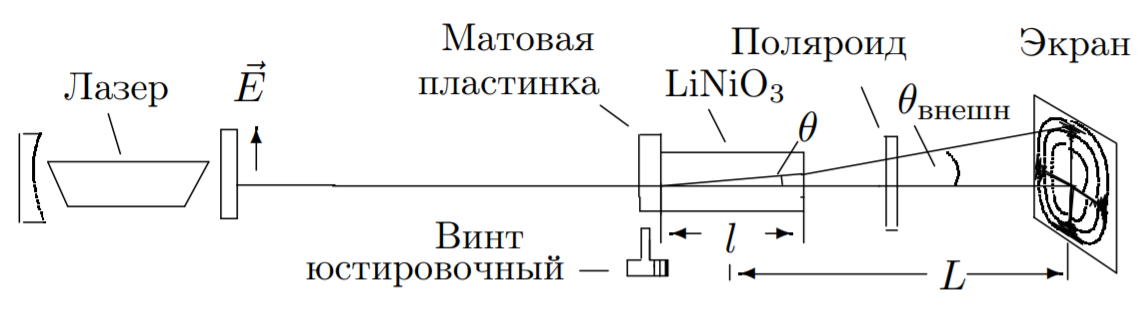
\includegraphics[width = 0.5\textwidth]{1.png}
\end{center}
\vspace{-20pt}
\caption{Схема для наблюдения интерфереционной картины.}
\end{wrapfigure}
%\begin{figure}[h!]
%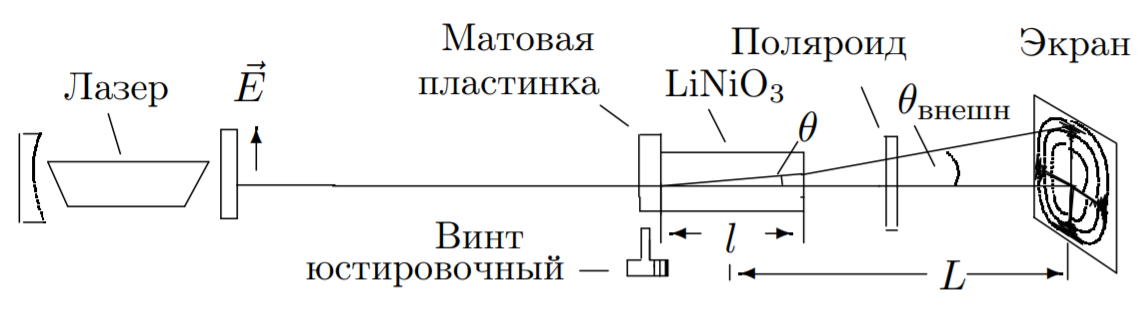
\includegraphics[scale=0.5]{1.png}
%\centering
%\caption{Схема для наблюдения интерфереционной картины}
%\end{figure}
Если перед кристаллом, помещённым между поляроидами, расположить линзу или матовую пластинку, то на экране за поляроидом мы увидим тёмные концентрические окружности -- рещультат интерфернции обыкновенной и необыкновенной волн. При повороте выходного поляроида на $90^\circ$ картина меняется с позитива на негатив (на месте светлых пятен тёмные и наоборот). В случаи, когда разрешённое направление анализатора перпендикулярно поляризации лазерного излучения, радиус тёмного кольца с номером $m$ равен
\begin{equation}
r_m^2 = \dfrac{\lambda}{l} \dfrac{(n_oL)^2}{n_0 - n_e}m,
\end{equation}

\begin{wrapfigure}{r}{0.45\textwidth}
\begin{center}
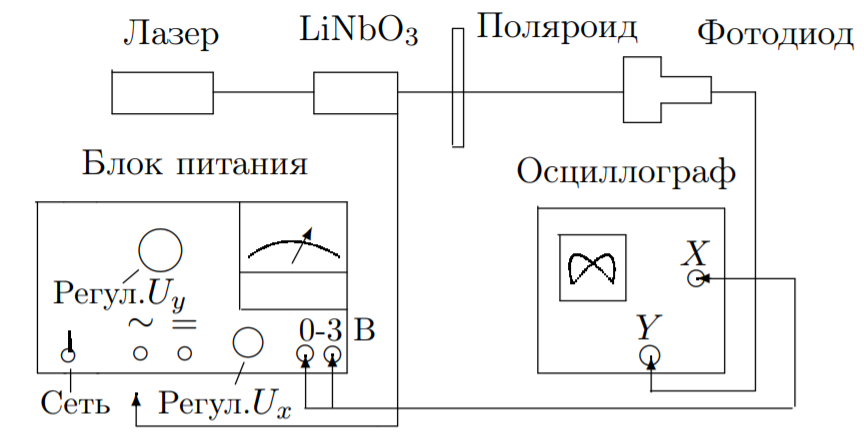
\includegraphics[width = 0.45\textwidth]{2.png}
\end{center}
\vspace{-20pt}
\caption{Схема установки.}
\end{wrapfigure}

где $L$ -- расстояние от центра кристалла до экрана, $l$ -- длина кристалла.\\
Теперь поместим кристалл в постоянное электрическое поле $E_{\text{эл}}$, направленное вдоль оси $X$, перпендикулярной $Z$. Показатель преломления для луча, распространяющего вдоль $Z$, всегда $n_o$. В плоскости $(X,Y)$ возникают два главных направления под углами $45^\circ$ к $X$ и $Y$ с показателями преломления $n_0 - \Delta n$ и $n_o + \Delta n$ (быстрая и медленная ось), причём $\Delta n = A E_{\text{эл}}$. Для поляризованного вертикально света и анализатора, пропускающего горизонтальную поляризацию, на выходе интенсивность на выходе будет иметь вид
\begin{equation}
I_{\text{вых}} = I_0 \sin^2 \left(\dfrac{\pi}{2} \dfrac{U}{U_{\lambda/2}} \right),
\end{equation}
где $U_{\lambda/2} = \frac{\lambda}{4A}\frac{d}{l}$ -- \textit{полуволновое напряжение}, $d$ -- поперечный размер кристалла.  При напряжении $U = E_{\text{эл}}d$ равном полуволновому сдвиг фаз между двумя волнами равен $\pi$, а интенсивность света на выходе максимальна. 


На Рис. 2 представлена схема всей установки (оптическая часть изорбажена на Рис. 1). Свет лазера, проходя через сквозь пластину, рассеивается и падает на двоякопреломляющий кристалл. На экране за поляроидом видна интерференционная картина. Убрав рассеивающую пластину и подавая на кристалл постоянное напряжение, можно величиной напряжения влиять на поляризацию луча, вышедшего из кристалла. Заменив экран фотодиодом и подав на кристалл переменное напряжение, можно исследовать поляризацию с помощью осциллографа.

\section*{Ход работы}
\subsection*{Определение разности показателей преломления}

\par Выполним юстировку системы. В схеме согласно Рис. 1 получим интерфереционную картину. 

\par Измерим радиусы $r(m)$ тёмных колец при расстоянии $L = 70 \pm 1 \text{ см}$ от середины кристалла до экрана. Результаты занесем в Таблицу 1. На Гр. 1 построим график $r^2 = f(m)$.

%\begin{wrapfigure}{r}{0.5\textwidth}
%\begin{center}
%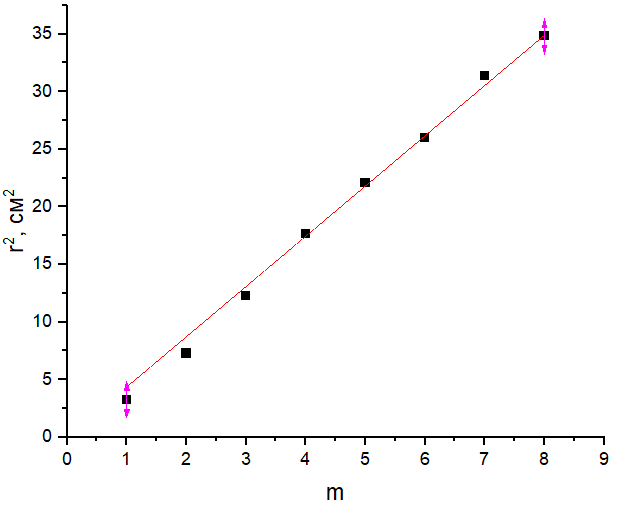
\includegraphics[width = 0.45\textwidth]{3.png}
%\end{center}
%\vspace{-40pt}
%\caption{Зависимость $r^2 = f(m)$.}
%\end{wrapfigure}
\begin{table}[h]
\begin{tabular}{|c|c|c|c|c|c|c|c|c|c|}
\hline
$m$     & 1   & 2   & 3   & 4   & 5   & 6   & 7   & 8   & 9 \\ \hline
$r_m$, см & 1.9 & 3.1 & 4 & 4.7 & 5.4 & 5.7 & 6.3 & 6.8 & 7.3 \\ \hline
\end{tabular}
\centering
\caption{Радиусы тёмных колец.}
\end{table}
\begin{center}
	\begin{tikzpicture}
	\begin{axis}[
	title={График 1 \quad Зависимость квадрата радиуса колец $r^2$ от их порядкового номера $m$},
	xlabel={$ m $},
	ylabel={$ r^2 $, см$^2$},
	legend pos=north west,
	xmajorgrids=true,
	ymajorgrids=true,
	grid style=dashed,
	width = 520,
	height = 350,
	%xmin = 300,
	%xmax = 335,
	%ymin =40,
	%ymax =0.22,
	]
	\legend{ 
		Результат измерений,
		Аппроксимация
	};
	\addplot+ [blue, only marks, mark size = 4pt,
	error bars/.cd,
	x dir=both, x explicit,
	y dir=both, y explicit, 
	] table [x = T, y = sigma] {
		T	sigma         
		1	3.61
        2	9.61
        3	16
        4	22.09
        5	29.16
        6	32.49
        7	39.69
        8	46.24
        9	53.29
	};
	\addplot [red, domain=0.5:9.5, line width =3.2pt] {6.1065 * x -2.5125};
	\end{axis}
	\end{tikzpicture}
\end{center}

При помощи аппроксимации методом хи-квадрат в программе OriginPro 2021 получаем угловой коэффициент $k = 6.1 \pm 0.1 \text{ см}^2$. Отсюда для значений $n_0 = 2.29$, $\lambda = 0.63 \text{ мкм}$, $l = 26 \text{ мм}$ получаем из формулы (2)
\[
\boxed{n_0 - n_e = 0.102 \pm 0.011}
\]  
\subsection*{Определение полуволнового напряжения}
\par Убедимся ещё раз, что направление лазерного луча совпадает с направлением на центр интерференционной картины и уберём матовую пластинку. Подключим разъём блока питания на постоянно напряжение, установим регулятор напряжения на минимум и включим блок питания в сеть.

Сначала определим интересующие нас напряжения без осциллографа. Для этого уберём матовую пластинку. При нулевом напряжении наблюдается минимум интенсиности излучения на экране. Постепенно увеличивая его, получим напряжение, соответстующее максимуму интенсивности $U_{\lambda/2} = (450 \pm 15) \text{ В}$.

Увеличивая напряжение далее определяем $U_\lambda$ и $U_{3\lambda/2}$:

\[U_\lambda = (900 \pm 30) \text{ В} \qquad U_{3\lambda/2} = (1350 \pm 45) \text{ В}\]

\par Подадим на кристалл напряжение $U_{\lambda/4} = \frac{1}{2}U_{\lambda/2}$. Вращая анализатор и наблюдая за яркостью пятна на экране, убеждаемся, что поляризация круговая.\\

Дальнейшие измерения проводим при помощи осциллографа. На установке по Рис. 2 определим полуволновое напряжение по разности напряжений при максимуме и минимуме у фигуры Лиссажу: \underline{$U_{\lambda/2} = 420 \pm 15 \text{ В}$}. 

Продолжая увеличивать напряжение получаем и другие величины $U_\lambda$ и $U_{3\lambda/2}$:

\[U_\lambda = (870 \pm 30) \text{ В} \qquad U_{3\lambda/2} = (1320 \pm 45) \text{ В}\]

Вид фигур Лиссажу для этих напряжений представлен в Таблице 2.

\begin{table}[h]
\centering
\begin{tabular}{|c|c|c|}
\hline
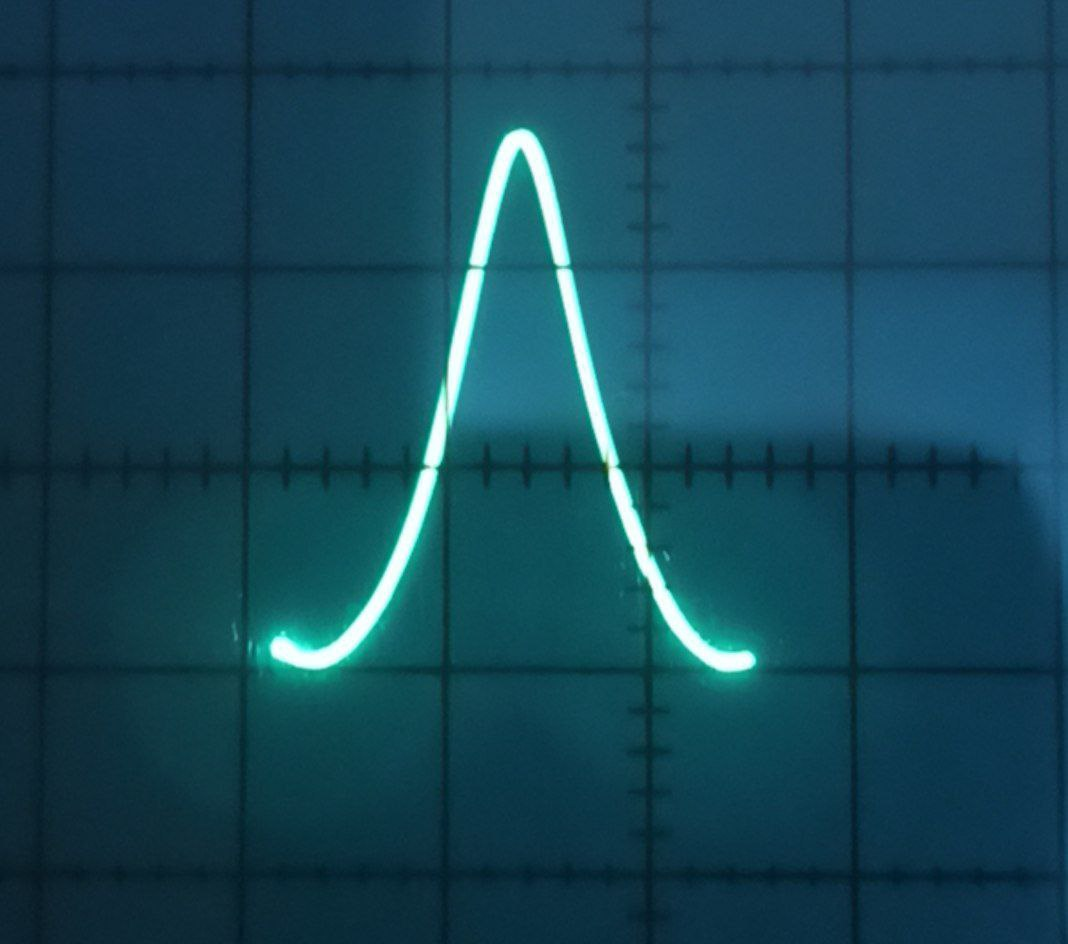
\includegraphics[height=4cm]{liss1.jpg}  & 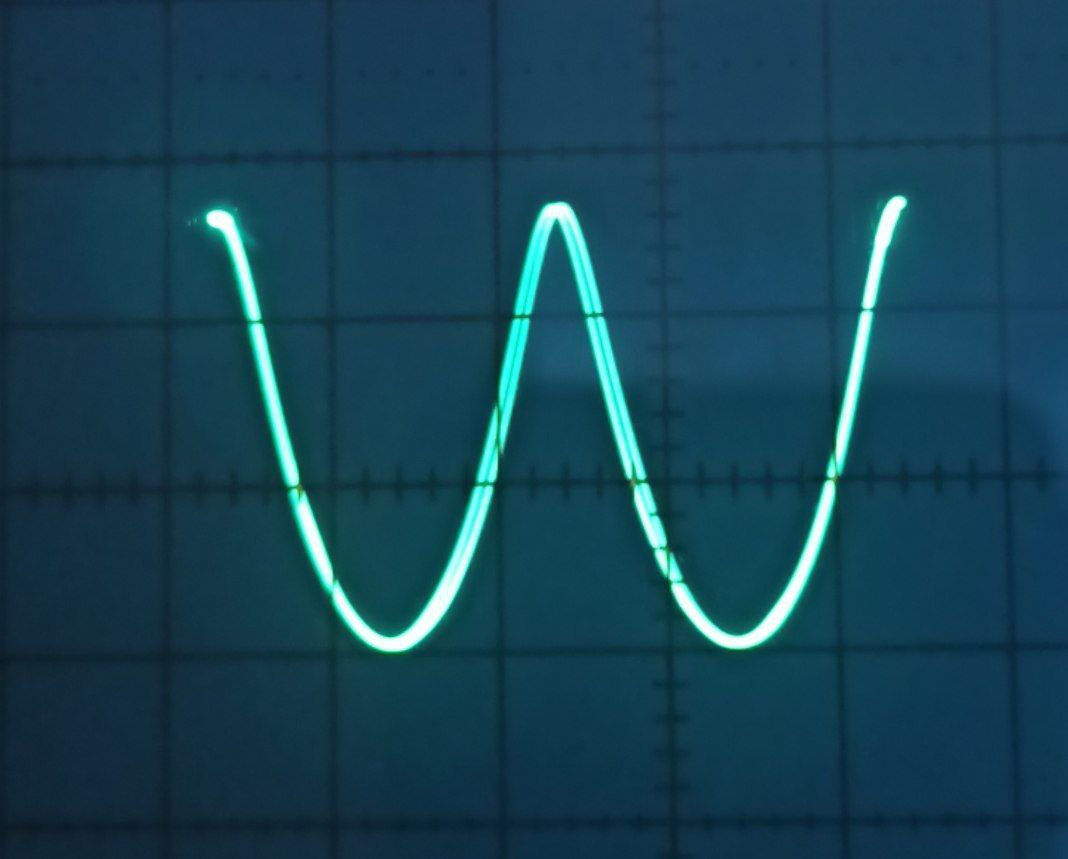
\includegraphics[height=4cm]{liss2.jpg}  &  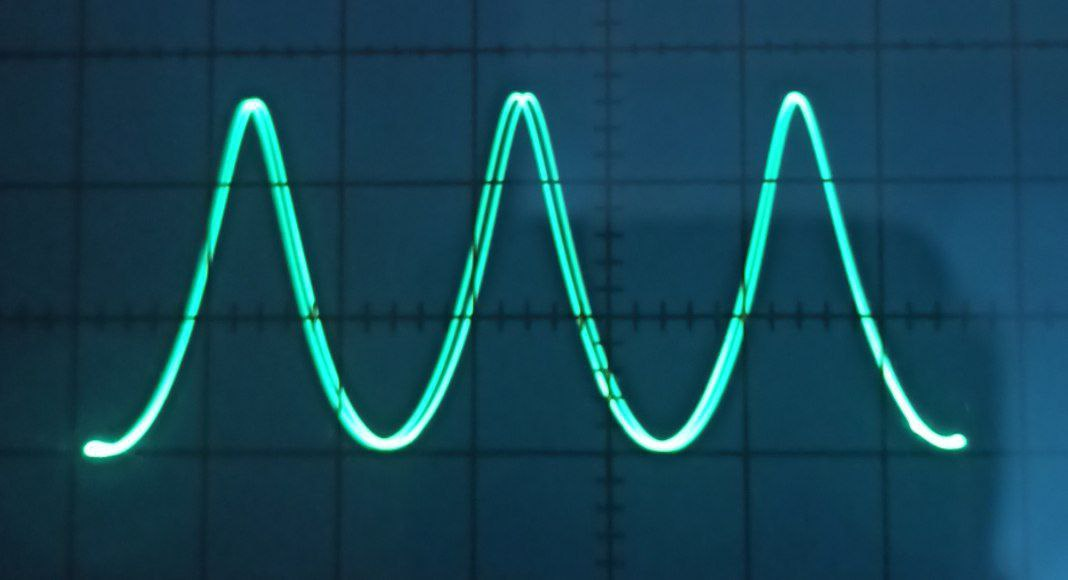
\includegraphics[height=4cm]{liss3.jpg} \\ \hline
$U_{\lambda/2}$ & $U_{\lambda}$ & $U_{3\lambda/2}$ \\ \hline
\end{tabular}
\caption{Фигуры Лиссажу для различных напряжений}
\label{tab:my-table}
\end{table}

\section*{Обсуждение результатов и выводы}
\begin{itemize}

\item Было проведено измерение радиусов тёмных колец $r(m)$ на расстоянии $L = 70 \pm 1 $ см от середины кристалла до экрана. Результаты приведены в Таблице 1. Из зависимости $r^2$ от порядкового номера кольца (График 1) аппроксимацией получили угловой коэффициент $k = 6.1 \pm 0.1 \text{ см}^2$. Отсюда для указанных на установке значений $n_0 = 2.29$, $\lambda = 0.63 \text{ мкм}$, $l = 26 \text{ мм}$ для двулучепреломления ниобата лития получили
\[
\boxed{n_0 - n_e = 0.10 \pm 0.01}
\]  
Табличное значение для двулучепреломления ниобата лития: $n_0 - n_e = 0.09$. Видим, что в пределах погрешности оно совпадает с полученным.

\item Было измерено полуполновое напряжение кристалла на длине волны $\lambda = 0.63 \text{мкм}$ при постоянном и переменном напряжениях. Первое определяем из условия максимума интенсивности, второе -- при помощи осциллографа по разности напряжений при максимуме и минимуме у фигуры Лиссажу. Получили 
\[
\boxed{U_{\lambda / 2}^{\text{AC}} = 450 \pm 15 \text{B}},
\boxed{U_{\lambda / 2}^{\text{DC}} = 420 \pm 15 \text{B}}
\]
Видим, что в пределах погрешности полученные значения совпадают.

\item Подав на кристалл четвертьволновое напряжение, вращая анализатор убедились в том, что поляризация на выходе из кристалла круговая.

\end{itemize}

Основоной вклад в ошибку в ходе выполнения работы могла внести неточность при определении диаметра колец на экране и выходного напряжения при помощи источника питания. Однако, порядок этой ошибки получился довольно приемлемым, что позволяет получить приемлемые результаты.

\end{document}